\paragraph{Vector Quantised Variational AutoEncoder (VQ-VAE) (2018)} \label{sec:vq-vae}

The \acf{VQ-VAE}, introduced in 2018, model distinguishes itself from traditional \acp{VAE} in two main aspects: the encoder network outputs discrete codes instead of continuous ones, and the prior is learned rather than static. While continuous feature learning has been the focus of many previous works, this model, introduced by \cite{oord_neural_2018}, concentrates on discrete representations, a natural fit for complex reasoning, planning, and predictive learning.

The \ac{VQ-VAE} model combines the \ac{VAE} framework with discrete latent representations through a parameterization of the posterior distribution of (discrete) latents given an observation. Based on vector quantization, this model is simple to train, does not suffer from significant variance, and avoids the ``posterior collapse''. As illustrated in Fig~\ref{fig:vq-vae}, the \ac{VQ-VAE} architecture consists of an encoder, a discrete latent space, and a decoder.

\begin{figure*}[ht]
    \centering
    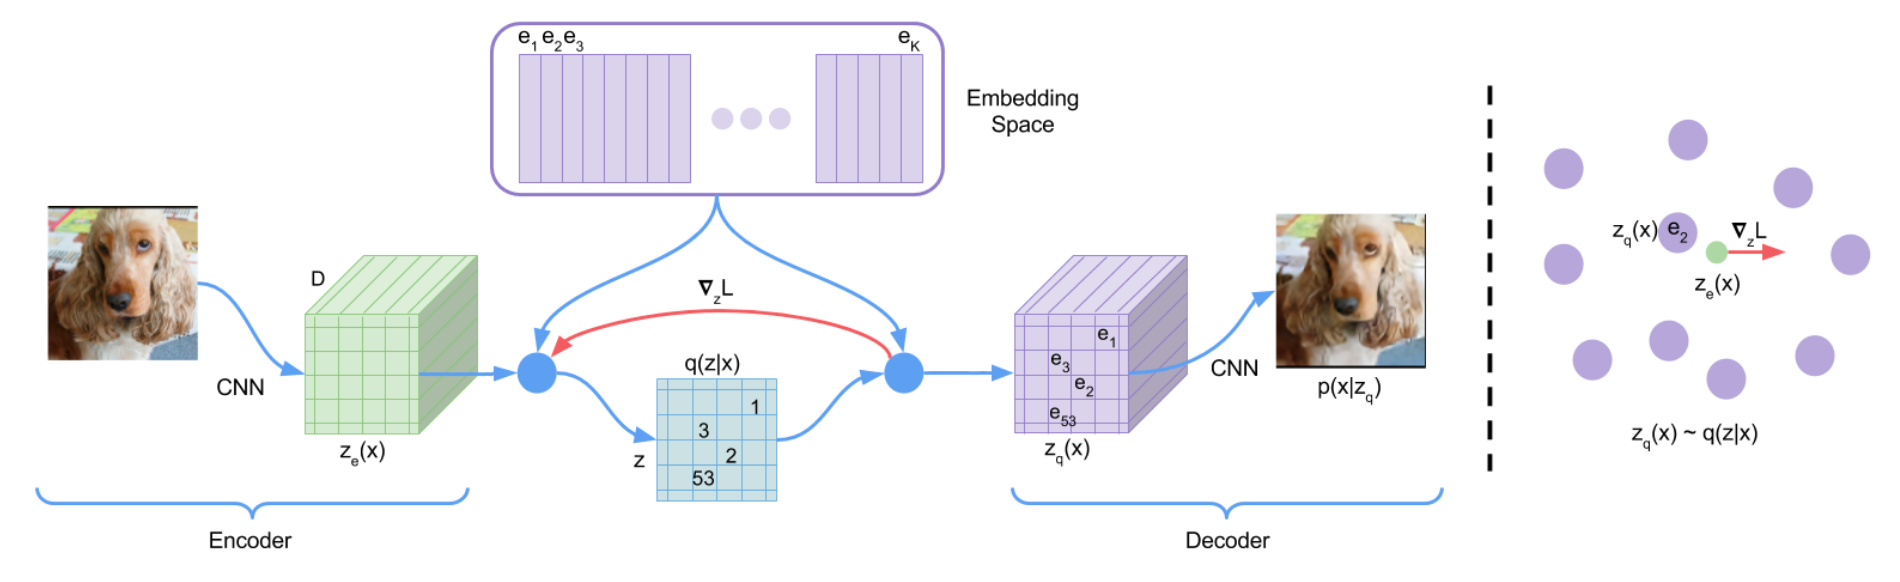
\includegraphics[width=\textwidth]{figures/2-sota/vq-vae.png}
    \caption[VQ-VAE]{\textbf{VQ-VAE} --- Taken from the original paper, this Figure presents two distinct illustrations. On the left side, a detailed diagram of the \ac{VQ-VAE} architecture is provided, showcasing the flow of information through the encoder, the discrete latent space, and the decoder. On the right side, a visualization of the embedding space is displayed, where the encoder output $z(X)$ is mapped to its nearest embedding point $e_2$. The red arrow represents the gradient $\nabla_z L$, influencing the encoder's output adjustment. This adjustment may result in a different configuration during the subsequent forward pass, highlighting the dynamic nature of the learning process within the \ac{VQ-VAE} model.}
    \label{fig:vq-vae}
\end{figure*}

The \ac{VQ-VAE} defines a latent embedding space $e \in R^{N \times D}$, where $N$ is the size of the discrete latent space (i.e., a $N$-way categorical), and $D$ is the dimensionality of each latent embedding vector $e_n$. There are $N$ embedding vectors $e_n \in R^D, n \in 1, 2, ..., N$. The model takes an input $X$, passed through an encoder producing output $z_e(X)$. The discrete latent variables $z$ are then calculated by the nearest neighbor look-up using the shared embedding space $e$. The input to the decoder is the corresponding embedding vector $e_n$. This forward computation pipeline is a regular autoencoder with a non-linearity that maps the latents to 1-of-N embedding vectors.

The posterior categorical distribution $q(z|X)$ probabilities are defined as one-hot (Eq. \ref{eq:vq-vae-posterior}):

\begin{equation} \label{eq:vq-vae-posterior}
  q(z = n|X) =
  \begin{cases}
    1 & \text{for } n = \text{argmin}_j ||z_e(X)-e_j||_2, \\
    0 & \text{otherwise}.
  \end{cases}
\end{equation}

where $z = e_n$ is the closest embedding vector to the encoder output $z_e(X)$. During forward computation, the nearest embedding $z_q(X)$ is passed to the decoder, and during the backward pass, the gradient $\nabla_z L$ is passed unaltered to the encoder. The overall loss function has three components to train different parts of the \ac{VQ-VAE}: the reconstruction loss, the \ac{VQ} objective, and the commitment loss. The total training objective becomes:

\setlength{\arraycolsep}{0.0em}
\begin{eqnarray}
\label{eq:vq-vae-loss}
\label{eq:reconstruction-loss}L&{}={}&\log p(X|z_q(X))\\
\label{eq:vq-objective}&&{+}\:||\text{sg}[z_e(X)] - e||_2^2\\
\label{eq:commitment-loss}&&{+}\:\beta||z_e(X) - \text{sg}[e]||_2^2
\end{eqnarray}
\setlength{\arraycolsep}{5pt}

This equation combines the three following terms:
\begin{enumerate}
	\item \textbf{Reconstruction loss} (Equation \ref{eq:reconstruction-loss}): This term represents the log probability of the input data $X$ given the latent variable  $z_q(X)$. It measures how well the model can reconstruct the input data using $z_q(X)$ as a representation. Maximizing this term would lead to a better reconstruction of the input data.
	\item \textbf{\Ac{VQ}} (Equation \ref{eq:vq-objective}): The second term measures the difference between the stop-gradient of the encoder output $z_e(X)$ and the embedding vector $e$. The stop-gradient operator, denoted as $\text{sg}$, acts as the identity during the forward pass but has zero partial derivatives during the backward pass. This term encourages the model to use the embeddings effectively by minimizing the distance between the encoder output and the closest embedding vector.
	\item \textbf{Commitment loss} (Equation \ref{eq:commitment-loss}): This term acts as a regularization term that measures the difference between the encoder output $z_e(X)$ and the stop-gradient of the embedding vector $e$. The  $\beta$ parameter controls the strength of this regularization. Minimizing this term would make $z_e(X)$  closer to the straight-through estimator of $e$.
\end{enumerate}

VQ-VAE has emerged as a vital component in generative artificial intelligence, spanning domains such as image~\cite{ramesh_zero-shot_2021} and sound generation~\cite{yang_diffsound_2022}.